\documentclass[11pt]{article}
\usepackage{amssymb,amsmath,amsthm,hyperref,verbatim,pict2e,graphicx,marvosym,array,booktabs,nameref}
\hypersetup{
	%colorlinks,citecolor=black,filecolor=black,linkcolor=black,urlcolor=black
	urlbordercolor=1 0 0,linkbordercolor=0 1 1, citebordercolor=0 1 1,
}
\usepackage[usenames]{xcolor} % color names ,dvipsnames,svgnames,table
\usepackage[utf8]{inputenc}
\usepackage[T1]{fontenc}
\usepackage[english]{babel}
\pagestyle{empty} % remove page numbers

\oddsidemargin 0.0cm
\evensidemargin 0.0cm
\topmargin 0.0cm
\headheight 0.0cm
\headsep 1.0cm
\textheight 21.0cm
\textwidth 16.0cm
\parskip 0.1cm
\parindent 0.0cm
\footskip 1.0cm

\usepackage[compact]{titlesec}
\titlespacing{\section}{0pt}{8pt}{0pt}
\titlespacing{\subsection}{0pt}{8pt}{0pt}
\titlespacing{\subsubsection}{0pt}{8pt}{0pt}
\usepackage{enumitem}
\setitemize{noitemsep,topsep=0pt,parsep=0pt,partopsep=0pt}
\setenumerate{noitemsep,topsep=0pt,parsep=0pt,partopsep=0pt}
\def\ul{\begin{itemize}}
\def\ule{\end{itemize}}
\def\ol{\begin{enumerate}}
\def\ole{\end{enumerate}}

% Recurrence visualisation helpers
\newcommand\Cd[3][0,-1]{\put(#2){\put(.5,.5){\circle*{.3}}\put(.5,.5){\linethickness{1.5pt}\vector(#1){#3}}}} % dependency [dx,dy]{x,y}{len}
\def\Cg#1{\put(#1){\color{lightgray}\put(0,0){\polygon*(0,0)(0,1)(1,1)(1,0)}}} % grayed cell (not to store
\def\Cz#1{\put(#1){\put(0,.35){\parbox{1\unitlength}{\centering\bf 0}}}} % zero-init cell
\def\Cm{\put(6.5,4.5){\circle*{.4}}\multiput(0,0)(1,0){9}{\line(0,1){8}}\multiput(0,0)(0,1){9}{\line(1,0){8}}} % matrix base
\def\Cfl#1{#1{0,6}#1{0,5}#1{1,5}#1{0,4}#1{1,4}#1{2,4}#1{0,3}#1{1,3}#1{2,3}#1{3,3}#1{0,2}#1{1,2}#1{2,2}#1{3,2}#1{4,2}
	#1{0,1}#1{1,1}#1{2,1}#1{3,1}#1{4,1}#1{5,1}#1{0,0}#1{1,0}#1{2,0}#1{3,0}#1{4,0}#1{5,0}#1{6,0}} % triangular lower (function)
\def\Cfd#1{#1{0,7}#1{1,6}#1{2,5}#1{3,4}#1{4,3}#1{5,2}#1{6,1}#1{7,0}} % main diagonal

\def\Cmlong{\put(6.5,4.5){\circle*{.4}}\multiput(0,0)(1,0){16}{\line(0,1){8}}\multiput(0,0)(0,1){9}{\line(1,0){15}}} % matrix base
\def\Cfu#1{#1{8,7}#1{9,7}#1{10,7}#1{11,7}#1{12,7}#1{13,7}#1{14,7}#1{9,6}#1{10,6}#1{11,6}#1{12,6}#1{13,6}#1{14,6}#1{10,5}#1{11,5}#1{12,5}#1{13,5}#1{14,5}#1{11,4}#1{12,4}#1{13,4}#1{14,4}#1{12,3}#1{13,3}#1{14,3}#1{13,2}#1{14,2}#1{14,1}} % triangular upper (function)

\title{DP Problems of Interest}
\author{Manohar Jonnalagedda, Thierry Coppey, Nithin George}
\date{}
\begin{document}
\maketitle
\pagestyle{headings}

% ----------------------------------------------------------------------------------------------------------------------------------------
\section{Introduction}
\subsection{Definitions}\ul
\item Block of computation: a block is simply a part of the DP matrix that we want to compute.
\item Wavefront: this is the place around which computation happen, typically. There should be some memory to store intermediate information between block of computations
\ule

\subsection{Problems classification}
In the literature, dynamic programming problems (DP) are classified according to two criteria:

\textbf{Monadic/polyadic}\ul
\item \textbf{Monadic:} on the right hand-side of the recurrence formula, only one term appears. For instance, Smith-Waterman with constant penalty is monadic
	\[M_{(i,j)}=\max\left\{\begin{array}{l} 0 \\ M_{(i-1,j-1)}+{\rm cost}(S(i),T(j))\\ M_{(i-1,j)}-d\\ M_{(i,j-1)}-d \end{array}\right. \]
\item \textbf{Polyadic:} when multiple terms of the recurrence occur in the right and-side of the recurrence formula. For instance Fibonacci is polyadic: \[F(n) = F(n-1) + F(n-2)\]
\ule

\textbf{Serial/non-serial} \ul
\item \textbf{Serial:} when the solution depends only of a fixed number of immediately previous solutions (i.e. neighbor cells). For instance Fibonacci is serial (it accesses only 2 cells backward).
\item \textbf{Non-serial:} when the solution depends of an arbitrary number of previous solutions. Typically Smith-Waterman with arbitrary gap penalty and Nussinov are non-serial:
	\[M_{(i,j)}=\max\left\{\begin{array}{l} ... \\ M_{(i,j-1)}\\ \max\limits_{i<k<j} [ M_{(i,k)}+M_{(k+1,j)} ] \end{array}\right. \]
\ule

\subsection{Simplifications}
\subsubsection{Calculus}
In some special case, it is possible to transform a non-serial problem into a serial problem, if we can embed the non-serial term into an additional aggregation matrix. For example:
	\[M_{(i,j)}=\max\left\{\begin{array}{l} \max\limits_{k<i} M_{(k,j)}
	\\ \sum\limits_{k<i, l<j}M_{(k,l)} \end{array}\right.
	\implies M_{(i,j)}=\max\left\{\begin{array}{l} C_{(k,j)} \\ A_{(i-1,j-1)} \end{array}\right.\]
Where the matrix $C$ stores the maximum along the column and matrix $A$ stores the sum of the array of the previous elements. Both can be easily computed with an additional recurrence:
	\[\begin{array}{rcl} C_{(i,j)}&=&\max(C_{(i-1,j)}, M_{(i,j)}) \\
	A_{(i,j)}&=&A_{(i-1,j)}+A_{(i,j-1)}-A_{(i-1,j-1)}+M_{(i,j)}\end{array}\]

This simplification avoids the non-serial dependencies at the cost of extra storage in the wavefront, unfortunately, it might be applicable only for some special cases.

\subsubsection{Precomputations}
When a calculus transformation is impossible, it might be worth to interleave a computation phase that will aggregate some of the results that are necessary to the computation block. For instance, for Nussinov term $\max_{i<k<j} [ M_{(i,k)}+M_{(k+1,j)} ]$, we can precompute it over all rows and columns of the block, and for all elements that are not part of the block, then pass these partial results together at the block launch to finish the computation.

On GPU, this could be done by interleaving a new kernel for this specific purpose, on FPGA, this could be done by preparing the maximums in another memory area whose pointer will later be passed to the co-processor. We may notice that since this phase is at the same time necessary for both architecture, and can be run independently, we can both execute them concurrently and mix between architectures (use CUDA for pre-computation and FPGA for actual tile computation for instance).

% ----------------------------------------------------------------------------------------------------------------------------------------
\section{Problems of interest}
We describe problems structures: inputs, cost matrices and backtracking matrix. These all have an alphabet (that must be bounded in terms of bit-size). Unless otherwise specified, we adopt the following conventions:\ul
\item Matrices dimensions are implicitly specified by number of indices and their number of elements is usually the same as the input length.
\item Number are all unsigned integers
\item Problem dimension is $m,n$ (or $n$) indices $i,j$ ranges are respectively $0\le i<m$, $0\le j<n$.
\item Unless otherwise specified, the recurrence applies to all non-initialized matrix elements.
\ule
We describe the problem processing in terms of both initialization and recurrences.

% ----------------------------------------------
\newpage
\subsection{Smith-Waterman (simple)}\label{sswat}\ol
\item Problem: matching two strings $S$, $T$ with $|S|=m, |T|=n$.
\item Matrices: $M_{m \times n}, B_{m \times n}$
\item Alphabets:\ul
	\item Input: $\Sigma(S)=\Sigma(T)=\{a,c,g,t\}$.
	\item Cost matrix: $\Sigma(M) = [0..z], z=\max({\rm cost(\_)}) \cdot \min(m,n)$
	\item Backtrack matrix: $\Sigma(B)=\{stop,W,N,NW\}$
	\ule
\item Initialization:\ul
	\item Cost matrix: $M_{(i,0)}=M_{(0,j)}=0$.
	\item Backtrack matrix: $B_{(i,0)}=B_{(0,j)}=stop$.
	\ule
\item Recurrence: \[M_{(i,j)}=\max\left\{\begin{array}{l|l}
		0 & stop\\
		M_{(i-1,j-1)}+{\rm cost}(S(i),T(j)) & NW\\
		M_{(i-1,j)}-d & N\\
		M_{(i,j-1)}-d & W
	\end{array}\right\}=B_{(i,j)} \]

\item Backtracking: starts from the cell $\max \{M_{(m,j)} \cup M_{(i,n)}\}$, stops at
the first cell containing a $0$.
\item Visualisation: by convention, we put the longest string vertically ($m\ge n$):
\begin{center}\setlength{\unitlength}{.6cm}\begin{picture}(8,9)
	\put(-.5,7.5){S}\put(-.35,7.4){\linethickness{1pt}\vector(0,-1){2}}
	\put(.2,8.2){T}\put(.8,8.4){\linethickness{1pt}\vector(1,0){2}}
	\Cz{0,0}\Cz{0,1}\Cz{0,2}\Cz{0,3}\Cz{0,4}\Cz{0,5}\Cz{0,6}\Cz{0,7}
	\Cz{1,7}\Cz{2,7}\Cz{3,7}\Cz{4,7}\Cz{5,7}\Cz{6,7}\Cz{7,7}
	\Cd{6,5}{0.8}
	\Cd[1,0]{5,4}{0.8}
	\Cd[1,-1]{5,5}{0.8}
\Cm\end{picture}\end{center}

\item Optimizations:\ul
	\item In serial (monadic) problems we can avoid building the matrix $M$ by only maintaining the 3 last diagonals in memory (one for the diagonal element, one for horizontal/vertical, and one being built). This construction extends easily to polyadic problems where we need to maintain $k+2$ diagonals in memory where $k$ is the maximum backward lookup.
	\ule
\ole

% ----------------------------------------------
\newpage
\subsection{Smith-Waterman (with gap extension at different cost)}\ol
\item Problem: matching two strings $S$, $T$ with $|S|=m, |T|=n$.
\item Matrices: $M_{m \times n}, E_{m \times n}, F_{m \times n}, B_{m \times n}$
\item Alphabets:\ul
	\item Input: $\Sigma(S)=\Sigma(T)=\{a,c,g,t\}$.
	\item Cost matrices: $\Sigma(M) = \Sigma(E) = \Sigma(F) = [0..z], z=\max({\rm cost(\_)}) \cdot \min(m,n)$
	\item Backtrack matrix: $\Sigma(B)=\{stop,W,N,NW\}$
	\ule
\item Initialization:\ul
	\item No gap cost matrix: $M_{(i,0)}=M_{(0,j)}=0$.
	\item T-gap extension cost matrix: $E_{(i,0)}= 0$ \textit{<<eat S chars only>>}
	\item S-gap extension cost matrix: $F_{(0,j)}= 0$
	\item Backtrack matrix: $B_{(i,0)}=B_{(0,j)}=stop$.
	\ule
\item Recurrence for the cost matrices:
\[\begin{array}{rcl}
M_{(i,j)}&=&\max\left\{\begin{array}{l|l}
	0 & stop\\
	M_{(i-1,j-1)}+{\rm cost}(S(i),T(j)) & NW\\
	E_{(i,j)} & N\\
	F_{(i,j)} & W
\end{array}\right\}=B_{(i,j)}\\
\\
E_{(i,j)}&=&\max\left\{\begin{array}{l|l}
	M_{(i, j-1)} - \alpha & NW\\
	E_{(i,j-1)} - \beta & N\\
\end{array}\right\}=B_{(i,j)}\\
\\
F_{(i,j)}&=&\max\left\{\begin{array}{l|l}
	M_{(i-1,j)} - \alpha & NW\\
	F_{(i-1,j)} - \beta & W\\
\end{array}\right\}=B_{(i,j)}
\end{array}\]

That can be written alternatively as:
\[M_{(i,j)}=\max\left\{\begin{array}{l|l}
	0 & stop\\
	M_{(i-1,j-1)}+{\rm cost}(S(i),T(j)) & NW\\
	\max_{1 \le k \le j-1} M_{(i,k)} - \alpha - (j-1-k) \cdot \beta & N\\
	\max_{1 \le k \le i-1} M_{(k,j)} - \alpha - (i-1-k) \cdot \beta & W\\
\end{array}\right\}=B_{(i,j)} \]

Although the latter notation seems more explicit, it introduces non-serial dependencies that the former set of recurrences is free of. So we need to implement the former rules whose kernel is 
\[ [M;E;F]_{(i,j)} = f_{\rm kernel} ( [M;E]_{(i,j-1)}, [M;F]_{(i-1,j)}, M_{(i-1,j-1)} ) \]
Notice that this recurrence is very similar to \nameref{sswat} except that we propagate 3 values ($M,E,F$) instead of a single one ($M$).

\item Backtracking: same as \nameref{sswat}
\item Visualisation: same as \nameref{sswat}
\item Optimizations: same as \nameref{sswat}
\ole

% ----------------------------------------------
\newpage
\subsection{Smith-Waterman with arbitrary gap cost}\label{aswat}\ol
\item Problem: matching two strings $S$, $T$ with $|S|=m, |T|=n$ with an arbitrary gap function $g(x)\ge 0$ where $x$ is the size of the gap. Without loss of generality, let $m\ge n$\footnote{Otherwise if $|T|>|N|$ we only need to swap both the inputs and backtracking pairs.}. Example penalty function could be\footnote{Intuition: long gaps penalize less, at some point, one large gap is better than matching and smaller gaps.} $g(x)=m-x$.
\item Matrices: $M_{m \times n}, B_{m \times n \times m}$
\item Alphabets:\ul
	\item Input: $\Sigma(S)=\Sigma(T)=\{a,c,g,t\}$.
	\item Cost matrix: $\Sigma(M) = [0..z], z=\max({\rm cost(\_)}) \cdot \min(m,n)$
	\item Backtrack matrix: $\Sigma(B)=\{stop,NW,N_{\{0..m\}},W_{\{0..n\}}\}$
	\ule

\item Initialization:\ul
	\item Match cost matrix: $M_{(i,0)}=M_{(0,j)}=0$.
	\item Backtrack matrix: $B_{(i,0)}=B_{(0,j)}=stop$.
	\ule

\item Recurrence:

\[M_{(i,j)}=\max\left\{\begin{array}{l|l}
	0 & stop\\
	M_{(i-1,j-1)}+{\rm cost}(S(i),T(j)) & NW\\
	\max_{1 \le k \le j-1} M_{(i,j-k)} - g(k) & N_k\\
	\max_{1 \le k \le i-1} M_{(i-k,j)} - g(k) & W_k\\
\end{array}\right\}=B_{(i,j)} \]


\item Backtracking: similar to \nameref{sswat} except that you can jump of $k$ cells.
\item Visualisation:

	\begin{center}\setlength{\unitlength}{.6cm}\begin{picture}(8,9)
		\put(-.5,7.5){S}\put(-.35,7.4){\linethickness{1pt}\vector(0,-1){2}}
		\put(.2,8.2){T}\put(.8,8.4){\linethickness{1pt}\vector(1,0){2}}
%		\Cd[0,1]{6,1}{2.8}\Cd[0,1]{6,2}{1.8}\Cd[0,1]{6,3}{0.8}
%		\Cd[1,0]{3,4}{2.8}\Cd[1,0]{4,4}{1.8}\Cd[1,0]{5,4}{0.8}
	\Cz{0,0}\Cz{0,1}\Cz{0,2}\Cz{0,3}\Cz{0,4}\Cz{0,5}\Cz{0,6}\Cz{0,7}
	\Cz{1,7}\Cz{2,7}\Cz{3,7}\Cz{4,7}\Cz{5,7}\Cz{6,7}\Cz{7,7}
		\Cd[0,-1]{6,7}{2.8}\Cd[0,-1]{6,6}{1.8}\Cd{6,5}{0.8}
		\Cd[1,0]{0,4}{5.8}\Cd[1,0]{1,4}{4.8}\Cd[1,0]{2,4}{3.8}\Cd[1,0]{3,4}{2.8}\Cd[1,0]{4,4}{1.8}\Cd[1,0]{5,4}{0.8}
		\Cd[1,-1]{5,5}{0.8}
	\Cm\end{picture}\end{center}

\item Optimizations: The dependencies here are non-serial, there is no optimization that we can 
apply out of the box here.
\ole


% ----------------------------------------------
\newpage
\subsection{Convex polygon triangulation}\ol
\item Problem: triangulating a polygon of $n$ vertices with least total cost for added edges. We denote the cost of adding an edge between the  pair of edges $i,j$ by $S(i,j)$, Where $S_{n \times n}$ is a lower triangular matrix compacted in memory (rows are contiguous) with a 0 diagonal that is omitted \footnote{Arbitrary convention for both architectural implementation and code generator. Rationale: in lower triangular matrix, element address is independent of the matrix size.}, hence $|S|=\tfrac{n^2}{2}=N$.

\item Matrices: $M_{n\times 2n}, B_{n \times 2n}$ \textit{<<first edge, last edge>>} upper triangular including main diagonal 
\item Alphabets:\ul
	\item Input: $\Sigma(S_{(i,j)})=\{0..m\}$ with $m=\max_S(i,j) \forall i,j$ determined at runtime\footnote{We need to scan/have stats about $S$ and that's where LMS plays a role}.
	\item Cost matrix: $\Sigma(M)=\{0..z\}$ with $z = m \cdot (n-2)$ (we add at most $n-2$ edges).
	\item Backtrack matrix: $\Sigma(B)=\{stop, 0..n\}$ (the index of the edge we add)
	\ule
\item Initialization: $M_{(i,i)}=0, M_{(i,i+1)}=0, B_{(i,i)}=stop \quad\forall i$

\item Recurrence: \[M_{(i,j)}=\left\{ \max_{i<k<j}M_{(i,k)}+M_{(k+1,j)} + S(i,k) \,\,\rule[-.75em]{.5pt}{2em}\,\,  k \right\} = B_{(i,j)} \]
	It is interesting to note that even in the sequential world, this problem is solved 
	by filling the diagonals, ie. computing sub-solutions for all polygons of size $k$ before
	those of size $k+1$.

\item Backtracking: Start at $B_{(1,n)}$. Use the following recursive function for the smaller polygons:
	\[{\rm BT}(B_{(i,j)}=k) \mapsto \left\{\begin{array}{ll} A_i & \text{if } k=0 \lor k=j \\
		\Big( {\rm BT}(B_{(i,k)}) \Big) \cdot \Big( {\rm BT}(B_{(k+1,j)}) \Big) & \text{otherwise} \end{array}\right.\]

\item Visualisation: the layout is the a matrix of size $n \times (2n-2)$, because of polygons being 
"cyclical" in nature.
\begin{center}\setlength{\unitlength}{.6cm}\begin{picture}(16,9)
	\put(-.7,6.5){\rotatebox{90}{First}}\put(-.4,6.4){\linethickness{1pt}\vector(0,-1){2}}
	\put(.2,8.2){Last}\put(1.5,8.4){\linethickness{1pt}\vector(1,0){2}}
	\Cfl{\Cg}\Cfd{\Cz}\Cfu{\Cg}
	\Cd[0,1]{6,1}{2.8}\Cd[0,1]{6,2}{1.8}\Cd[0,1]{6,3}{0.8}
	\Cd[1,0]{3,4}{2.8}\Cd[1,0]{4,4}{1.8}\Cd[1,0]{5,4}{0.8}
	\put(3.5,4.5){\line(3,-1){3}}
	\put(4.5,4.5){\line(2,-2){2}}
	\put(5.5,4.5){\line(1,-3){1}}
	%\Cd[1,-1]{5,2}{0.8}
\Cmlong\end{picture}\end{center}

\item Optimizations: we need to rotate that matrix to progress in the same direction as usual, that is towards bottom right.
{\color{red}}
\ole


% ----------------------------------------------
\newpage
\subsection{Matrix chain multiplication}\ol
\item Problem: find an optimal parenthesizing of the multiplication of $n$ matrices $A_i$. Each matrix $A_i$ is of dimension $r_i \times c_i$ and $c_i=r_{i+1} \forall i$. \textit{<<r=rows, c=columns>>}
\item Matrices: $M_{n \times n}, B_{n \times n}$ \textit{(first, last matrix)}
\item Alphabets:\ul
	\item Input: matrix $A_i$ size is defined as pairs of integers $(r_i,c_i)$.
	\item Cost matrix: $\Sigma(M):=$ huge integer\footnote{Integer multiplication might blow up, use float or doubles and addition of logarithms instead.}.
	\item Backtrack matrix: $\Sigma(B)=\{stop\} \cup \{0..n\}$.
	\ule
\item Initialization:\ul
	\item Cost matrix: $M_{(i,i)}=0$.
	\item Backtrack matrix: $B_{(i,i)}=stop$.
	\ule
\item Recurrence: $c_k=r_{k+1}$
	\[M_{(i,j)}=\min_{i\le k<j}\left\{\begin{array}{l|l}
		M_{(i,k)}+M_{(k+1,j)}+r_i \cdot c_k \cdot c_j & k
	\end{array}\right\}=B_{(i,j)} \]
\item Backtracking: Start at $B_{(1,n)}$. Use the following recursive function for parenthesizing
	\[{\rm BT}(B_{(i,j)}=k) \mapsto \left\{\begin{array}{ll} A_i & \text{if } k=0 \lor k=j \\
		\Big( {\rm BT}(B_{(i,k)}) \Big) \cdot \Big( {\rm BT}(B_{(k+1,j)}) \Big) & \text{otherwise} \end{array}\right.\]

\item Visualisation:
	\begin{center}\setlength{\unitlength}{.6cm}\begin{picture}(8,9)
		\put(-.7,6.5){\rotatebox{90}{First}}\put(-.4,6.4){\linethickness{1pt}\vector(0,-1){2}}
		\put(.2,8.2){Last}\put(1.5,8.4){\linethickness{1pt}\vector(1,0){2}}
		\Cfl{\Cg}\Cfd{\Cz}
		\Cd[0,1]{6,1}{2.8}\Cd[0,1]{6,2}{1.8}\Cd[0,1]{6,3}{0.8}
		\Cd[1,0]{3,4}{2.8}\Cd[1,0]{4,4}{1.8}\Cd[1,0]{5,4}{0.8}
		\put(3.5,4.5){\line(3,-1){3}}\put(4.5,4.5){\line(2,-2){2}}\put(5.5,4.5){\line(1,-3){1}}
	\Cm\end{picture}\end{center}

\item Optimizations:\ul
	\item {\color{red}We need to swap vertically the matrix to have a normalized progression towards bottom right. To do that, we need to map all indices $i \mapsto n-1-i$, but since we want to store the matrix sparsely, we might want to transform it into a lower triangular matrix as we can provide a size-independent mapping of element indices.
	XXX: what's the best trade off ? progress towards bottom right VS map indices more efficiently ?}
	\ule
\ole

% ----------------------------------------------
\newpage
\subsection{Nussinov algorithm}\ol
\item Problem: folding a RNA string $S$ over itself $\left\lfloor |S| / 2 \right\rfloor = n$.
\item Matrices: $M_{n\times n}, B_{n \times n}$
\item Alphabets:\ul
	\item Input: $\Sigma(S)=\{A,C,G,U\}$.
	\item Cost matrix: $\Sigma(M)=\{0..n\}$
	\item Backtrack matrix: $\Sigma(B)=\{stop,D,1..n\}$
	\ule
\item Initialization: \ul
	\item Cost matrix: $ M_{(i,i)}=M_{(i,i-1)}=0$
	\item Backtrack matrix: $B_{(i,i)}=B_{(i,i-1)}=stop$
	\ule
\item Recurrences:
	\[M_{(i,j)}=\max\left\{\begin{array}{l|l}
		M_{(i+1,j-1)}+\omega(i,j) & D\\
		\max_{i\le k<j}M_{(i,k)}+M_{(k+1,j)} & k
	\end{array}\right\} = B_{(i,j)} \]
	With $\omega(i,j)=1$ if $i,j$ are complementary. 0 otherwise.
\item Backtracking: Start the backtracking in $B_{(1,n)}$ and go backward. The backtracking is very similar to that of the matrix multiplication, except that we also introduce the diagonal matching.
\item Visualisation:
	\begin{center}\setlength{\unitlength}{.6cm}\begin{picture}(8,9)
		\put(-.7,6.5){\rotatebox{90}{First}}\put(-.4,6.4){\linethickness{1pt}\vector(0,-1){2}}
		\put(.2,8.2){Last}\put(1.5,8.4){\linethickness{1pt}\vector(1,0){2}}
		\Cfl{\Cg}\Cfd{\Cz}
		\Cd[0,1]{6,1}{2.8}\Cd[0,1]{6,2}{1.8}\Cd[0,1]{6,3}{0.8}
		\Cd[1,0]{3,4}{2.8}\Cd[1,0]{4,4}{1.8}\Cd[1,0]{5,4}{0.8}
		\Cd[1,1]{5,3}{0.8}
		\put(3.5,4.5){\line(3,-1){3}}\put(4.5,4.5){\line(2,-2){2}}\put(5.5,4.5){\line(1,-3){1}}
	\Cm\end{picture}\end{center}

\item Optimizations: note that this is very similar to the matrix multiplication except that we also need the diagonal one step backward, so the same optimization can apply.
\ole

% ----------------------------------------------
\newpage
\subsection{Zuker folding}\ol
\item Problem: folding a RNA string $S$ over itself $\left\lfloor |S| / 2 \right\rfloor = n$.
\item Matrices: $V_{n\times n}, W_{n\times n}, F_n$ (Free Energy),  $BV_{n \times n}, BW_{n \times n}, BF_n$
\item Alphabets:\ul
	\item Input: $\Sigma(S)=\{A,C,G,U\}$.
	\item Cost matrices:\ul
		\item $\Sigma(W)=\Sigma(V)=\{0..z\}$ with $z \le n*b+c$
		\item $\Sigma(F)=\{0..y\}$ with $y\le \min(F_0, z\cdot n)$
		\ule
	\item Backtrack matrices: \ul
		\item $\Sigma(BW)=\{stop, S,W,V,k\}$
		\item $\Sigma(BV)=\{stop, HL, IL, SW, (i,j) , k\}$ with $0\le i,j,k < n$ \\
		$HL$=HairpinLoop, $IL$=InteriorLoop, $(i,j)$=MultiLoop
		
		
		\item $\Sigma(BF)=\{stop, L, k\}$ with $0\le k < n$
		\ule
	\ule
\item Initialization:\ul
	\item Cost matrices: $W_{(i,i)}=V_{(i,i)}=0, F_{(0)}=$ energy of the unfolded RNA.
	\item Backtrack matrices: $BW_{(i,i)}=BV_{(i,i)}=BF_{(0)}=stop$.
	\ule
\item Recurrence:
\[\begin{array}{rcl}
W_{(i,j)}&=&\min\left\{\begin{array}{l|l}
	W_{(i+1,j)}+b & S\\
	W_{(i,j-1)}+b & W\\
	V_{(i,j)}+\delta(S_i,S_j) & V \\
	\min_{i<k<j}W_{(i,k)}+W_{(k+1,j)} &k
\end{array}\right\} = BW_{(i,j)}\\
\\
V_{(i,j)}&=&\min\left\{\begin{array}{l|l}
	\infty \qquad\qquad\qquad\qquad {\rm if}(S_i,S_j) \text{ is not a base pair} & stop\\\\
	eh(i,j)+b \qquad\qquad\, \text{otherwise} & HL\\
	V_{(i+1,j-1)}+es(i,j) & IL \\
	VBI(i,j) & (i',j') \\
	\min_{i<k<j-1}\{W_{(i+1,k)}+W_{(k+1,j-1)}\} +c & k
\end{array}\right\} = BV_{(i,j)}\\
\\
F_{(j)}&=&\min\left\{\begin{array}{l|l}
	F_{(j-1)} & L \\ 
	\min_{1\le i< j} (F_{(i-1)} + V_{(i,j)}) & i
\end{array}\right\} = BF_{(j)}\\
\\
VBI(i,j)&=&\min_{i<i'<j'<j}\{V_{(i',j')}+ebi(i,j,i',j')\} +c \quad|\quad (i',j')=BV_{(i,j)}
\end{array}\]

In practice, we don't go backward for larger values than 30, so we can replace $\min_{i<k<j}$ by $\min_{\max(i,j-30)<k<j}$ in the expressions of $W$,$V$, $VBI$ and $F$.

{\color{red}
\item Backtracking: Start at $BF_{(n)}$ using the recurrences
 \[\begin{array}{rcl}
	BF_{(j)} &=& \left\{\begin{array}{rcl} L&\implies& BF_{(j-1)} \\ i &\implies& BF_{(i-1)} + BV_{(i,j)} \end{array} \right.\\
	\\
	BV(i,j) &=& \left\{\begin{array}{rcl}
		HL &\implies&\big< {\rm hairpin}(i,j) \big> \\
		IL &\implies& \big< {\rm stack}(i,j) \big> BV_{(i+1,j-1)} \\
		(i',j') &\implies& \big< \text{multi-loop from $(i,j)$ to }(i',j') \big> BV(i',j')\\
		k &\implies& BW_{(i+1,k)} BW_{(k+1,j-1)}
	\end{array}\right.\\
	\\
	BW_{(i,j)} &=& \left\{\begin{array}{rcl}
	S & \implies & \big< bulge(i) \big> BW_{(i+1,j)} \\
	W & \implies & \big< bulge(j) \big> BW_{(i,j+1)} \\
	V &\implies& BV_{(i,j)} \\
	k &\implies& BW_{(i+1,k)} BW_{(k+1,j-1)}
	\end{array}\right.
\end{array}\]
}
\item Visualisation: \begin{center}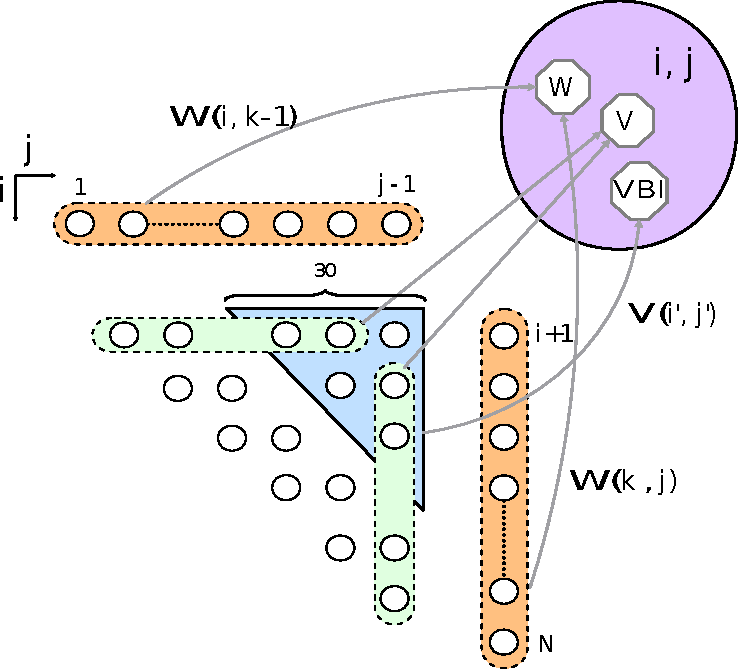
\includegraphics[width=7cm]{problems_zucker.pdf}\end{center}
	% source: <<Parallization of dynamic programming recurrences in computational biology>> paper
\item Optimizations: {\color{red} XXX}
\ole

% ------------------------------------------------------------------------------------------------
\newpage
\section{Plan}
\ol
\item \textbf{Problems:} finish the problem description. \\ We might look towards parallel tree-raking, but it does not share much with the above algorithms (sparse version of above computations, might not scale that well). Most of the common patterns are already enclosed by the above problems. Real input size is around 300'000 (we may want to target the million, using disk). We might want to also look at an $O(n^3)$-space complexity problem (like matching 3 strings $S,T,U$).
\item \textbf{User facing language:} goals are flexibility and compactness.\ul
	\item Design the user-facing language that we want to support, which should be similar to related papers <<Algebraic Dynamic Programming>> and <<ADP fusion>>. We want to reuse their transformation to map (problem description) $\mapsto$ (kernel implementation) for a single element.
	\item We also may want to try to make implicit transformation for code like \\
		{\tt @DP def Fib(n:Int) = if (n<=2) return 1 else Fib(n-1)+Fib(n-2)}.
	\item Windowing: the user should be able to force a windowing (i.e. force a non-serial problem to be a $k$-polyadic serial problem).	
	\item Consider 3 different cases: we care about backtrack, the costs or both.
	\item Backtracking: we might want to create an operator/class that given an item produces the previous in the backtrack, or the whole sequence in correct order, or only indices.
	\ule
Get an implementation by \emph{end of October}.

\item \textbf{Prototyping:} get a prototype to understand difficulties and share common base. \\ Implement a working prototype of \nameref{aswat} on CPU (for correctness), and specific platform (CUDA/FPGA). This will give us an idea of how to implement the general case. We also need to benchmark and compare both implementations to see how we compare to existing implementations and see the direction to take (which decide is faster and by how much). Here we aim to do as good an implementaion for the specific platform (CPU/GPA) as possible.

\item \textbf{Baseline:} get some implementations working on the different platforms and use them as baselines. Goal to get something working by \emph{end of October}.

\item \textbf{Formalize IR:} According to experiences, describe the intermediate representation, also formalize the framework that will be provided to the code generators (i.e. memory management, ...).
\item \textbf{Full compiler stack:} enrich the compiler stack from both top-down (translate best user-facing language parsers) and bottom-up (parametric code generators), core of the work.
\item \textbf{Test and benchmark:} make sure our implementations are correct and compare them with previous papers implementations.
\ole

\newpage
\subsection{LMS compiler stack}
\textbf{User-language}: define additional parameters for the recurrence\ul
\item Windowing (to convert non-serial into serial problems)
\item Input sizes, and alphabets (backtrack, input, cost)
\item Backtrack (implicitly by backtrack alphabet size) and cost matrices bit-sizes (cost maximum may be inferred using <<Yield size/grammar analysis>>)
\item Recurrence functions, devices available
\item What to keep in memory (cost, backtrack or both).
\ule
$\Downarrow$ Conversion (using an existing technique)

\textbf{Intermediate representation}

$\Downarrow$ Optimizations\ul
\item Transform non-serial into serial \ul
	\item Use aggregation functions/transformations
	\item Use windowing from user (if no other technique succeed)
	\ule
\item Define the wavefront depth
\item Avoiding the cost matrix by moving it into the wavefront
\ule

\textbf{Code specification}\ul
\item Kernel function (1-element function), inputs, outputs, wave front, dependencies, bit sizes
\item Device-level interface => setup the block sizes(w/h), input and memory sizes
\item Define the device-specific implementation of the block (CPU/FPGA/CUDA)
\item Define the co-processor memory aggregation function
\item Define the scheduling of the blocks and aggregation (software pipelining)
\item Define the data movement back and forth to disk
\ule

$\Downarrow$ Generation\ul
\item Generate the kernel for specific device
\item Generate the scheduling and barriers
\ule

\textbf{Binary program}

%\ol
%\item Make sure we encompass all the most common patterns of DP: check if we have higher dimensions or more complex formula.
%\item Let the user tune the window size if he wants to reduce non-serial to serial.
%\item Concerns separation: common architecture enables flexibility (exchange components) \ul
%	\item Block processor: CPU, GPU, FPGA, must allow variation of width and height
%	\item Memory stats computation (min, sum, ... column/line combinations): CPU, GPU
%	\item Scheduler (CPU): interleave block computation and memory statistics
%	\ule
%\item Common description \ul
%	\item Block kernel processor
%	\item Full block
%	\ule
%\item Discussion: wavefront, design similarities, polyhedral theory
%\ole

%%\newcolumntype{C}[1]{>{\centering\let\newline\\\arraybackslash}m{#1}}
%\newcolumntype{C}{@{\hspace{7pt}}c@{\hspace{7pt}}}
%\def\mnl{\rule{0pt}{2.6ex}\rule[-1.2ex]{0pt}{0pt} \\ \hline}
%$\begin{array}{|C|C|C|C|C|C|} \hline
%0 & 0 & 0 & 0 & 0 & 0 \mnl
%0 &  &  &  &  & \mnl
%0 & M_{23}  &  &  &  & \mnl
%0 &  & \sum  &  &  & \mnl
%0 &  &  &  &  & \mnl
%0 &  &  &  &  & \mnl
%\end{array}$
\end{document}
